
% basic settings: 
%%%%%%%%%%%%%%%%%%%%%%%%%%%%%%%%%%%%%%%%%%%%%%%%%%%%%%%%%%%%%%%%%%%%%%%%%%%%%%%%%%%
\documentclass[11pt]{article}
\usepackage[a4paper,margin=2.8cm]{geometry}
\usepackage[ansinew]{inputenc}


% packages:
%%%%%%%%%%%%%%%%%%%%%%%%%%%%%%%%%%%%%%%%%%%%%%%%%%%%%%%%%%%%%%%%%%%%%%%%%%%%%%%%%%%
\usepackage[english]{babel}
\usepackage{enumerate}  
\usepackage[shortlabels]{enumitem} 
\usepackage{amsmath}
\usepackage{amsthm}
\usepackage{empheq} % enhanced amsmath environment, allows to put things into modified boxes, brackets etc. 
\usepackage{amssymb}
\usepackage[pdftex]{graphicx}
\usepackage[dvipsnames,usenames]{color} % to have colored text
\usepackage[colorlinks=true,linkcolor=NavyBlue,citecolor=NavyBlue,urlcolor=NavyBlue]{hyperref} % for hyperlinks 
\usepackage{authblk} % for author affiliations
\usepackage{cite} % to have well-formatted citations
\usepackage{appendix}


%%% bibliography settings
%%%%%%%%%%%%%%%%%%%%%%%%%%%%%%%%%%%%%%%%%%%%%%%%%%%%%%%%%%%%%%%%%%%%%%%%%%%%%%%%%%%
\usepackage{natbib}
\bibliographystyle{humannat}
\setcitestyle{authoryear}
\setlength{\bibsep}{1pt}

% makros:
%%%%%%%%%%%%%%%%%%%%%%%%%%%%%%%%%%%%%%%%%%%%%%%%%%%%%%%%%%%%%%%%%%%%%%%%%%%%%%%%%%%%
\newcommand{\nt}[3]{\int \limits_{#1}^{#2} \mathrm{d}#3~} % integral with boundaries
\newcommand{\dd}{\mathrm{d}} % differential d

% Title, authors and affiliations
%%%%%%%%%%%%%%%%%%%%%%%%%%%%%%%%%%%%%%%%%%%%%%%%%%%%%%%%%%%%%%%%%%%%%%%%%%%%%%%%%%%
\title{\texttt{SDE\_DensityTracking} \\ A Python Package}
\author{}
\date{}
%%%%%%%%%%%%%%%%%%%%%%%%%%%%%%%%%%%%%%%%%%%%%%%%%%%%%%%%%%%%%%%%%%%%%%%%%%%%%%%%%%%


\begin{document}
\maketitle
%%%%%%%%%%%%%%%%%%%%%%%%%%%%%%%%%%%%%%%%%%%%%%%%%%%%%%%%%%%%%%%%%%%%%%%%%%%%%%%%%%%

The implementation consists of one single class that tracks the density distribution of the solution to a stochastic differential equation (SDE). 
Starting from a generic SDE
\begin{equation}
	\dd X_t = \mu(X_t)~ \dd t + \sigma(X_t) ~\dd W_t
	\label{eq:SDE_generic}
\end{equation}
with some time-independent drift and volatility functions $\mu$ and $\sigma$, and initial position $X_0$, 
the class calculates the probability density $p(x,t)$, to be at position $x$ at time $t$. 
The class can furthermore deal with absorbing or reflective boundary conditions. 


\section{Input \& Output} 
%%%%%%%%%%%%%%%%%%%%%%%%%%%%%%%%%%%%%%%%%%%%%%%%%%%%%%%%%%%%%%%%%%%%%%%%%%%%%%%%%%%

Upon initialization of the class with appropriate arguments, 
one starts tracking the evolution of the density by calling the \texttt{track\_density} method. 
Once finished, the density $p = p(x,t)$ can be retrieved by calling the \texttt{get\_density} method. 
The return value can be either a functional or discretized object, and it can be either a function of $x$, of $t$, or both. 
See documentation inside \texttt{SDE\_DensityTracking.py} for a detailed description of all input and output values. 


\section{Theoretical Background} 
%%%%%%%%%%%%%%%%%%%%%%%%%%%%%%%%%%%%%%%%%%%%%%%%%%%%%%%%%%%%%%%%%%%%%%%%%%%%%%%%%%%

In our implementation, we have followed the approach of \cite{Bhat2016}, which is straight forward. 
We first discretize \eqref{eq:SDE_generic} in time, giving
\begin{equation}
	X_{t+1} = X_t +  \mu(X_t) \Delta t + \sigma(X_t) \sqrt{ \Delta t} Z_t
	\label{eq:SDE_generic_discretized}
\end{equation}
with $\Delta t$ the discretization step width and $Z_t$ a normally distributed random variable. 
Looking at \eqref{eq:SDE_generic_discretized}, we can see immediately that the position of $X_{t+1}$ is just a 
Gaussian with mean $X_t +  \mu(X_t) \Delta t$ and standard deviation $\sigma(X_t) \sqrt{ \Delta t}$. 
Let us denote by $G(x,y)$ a Gaussian with mean $y+\mu(y) \Delta t$ and standard deviation $\sigma(y) \sqrt{ \Delta t}$. 
Then, the density at position $x$ at time $t+1$ is just given by the Chapman-Kolmogorov equation 
\begin{equation}
	p(x, t+1) = \int_{\mathbb{R}} \dd y ~ G(x, y) ~ p(y, t). 
	\label{eq:CK}
\end{equation}
Discretizing \eqref{eq:CK} yields 
\begin{equation}
	p(x, t+1) \approx k  \sum_{i=-\infty}^\infty  \dd y ~ G(x, y) ~ p(y_i, t). 
	\label{eq:CK_discrete}
\end{equation}
where $k$ is the spatial discretization step, ie. $k = y_{i+1}-y_i ~ \forall i$. 
For the numerical implementation, the infinite sum in \eqref{eq:CK_discrete} is truncated naturally by just summing over all values $y_i$ calculated at time $t$. 
The considered value range $x_i$ at time $t+1$ is determined dynamically at runtime as the minimum and maximum value below and above
which the density is less than some pre-specified precision value \texttt{tol}, that we can safely approximate as zero. 
\footnote{
In principle, this implementation can cause some problem in case of a a bimodal initial distribution with two unconnected peaks, 
i.e. with regions of zero probability mass between the two peaks. 
Because this is a very specific case, we ignore it for here for simplicity. 
} 
This new range of values at time $t+1$ naturally truncates the summation in \eqref{eq:CK_discrete} in the next iteration, and so on. 
If there is an absorbing boundary, we must just replace the Gaussian $G(x,y)$ in \eqref{eq:CK_discrete} by 
\begin{align}
	p(s, t ~ ; ~s_0, \underline{s}=0) = \frac{1}{\sqrt{2 \pi \sigma^2 t}} &
 							\left[
 							 \exp \left( - \frac{ ( s_0 + \mu t - s )^2 }{2 \sigma^2 t}   \right) \right.  \notag \\
							 &~~~~							 
 							\left.  - \exp \left( - \frac{2 s_0 \mu}{\sigma^2} \right) 
							 \exp \left(- \frac{  ( s_0 - \mu t + s )^2 }{2 \sigma^2 t} \right) 							 
 							 \right],
							 \label{eq:p_absorbing_explicit}
\end{align} 
which is the density of a random walk with drift $\mu$ and volatility $\sigma$, in presence of an absorbing boundary at $s = 0$. 
A formula similar to equation \eqref{eq:p_absorbing_explicit} exists for the reflective barrier. 
See for  instance \cite{Molini2011} for a derivation of these results. 

Note that technically, we are not solving the Fokker-Planck equation, but the Chapman-Kolmogorov forward equation. 
This implementation has the additional advantage that the range of $x$-values is dynamic (no previous grid must be specified), 
and $\mu$ and $\sigma$ must not necessarily be differentiable. 


\section{Consistency check} 
%%%%%%%%%%%%%%%%%%%%%%%%%%%%%%%%%%%%%%%%%%%%%%%%%%%%%%%%%%%%%%%%%%

We have checked the validity of the implementation in figure \ref{fig:PDE_solution}. 
\begin{figure}[!htb]
	\centering
	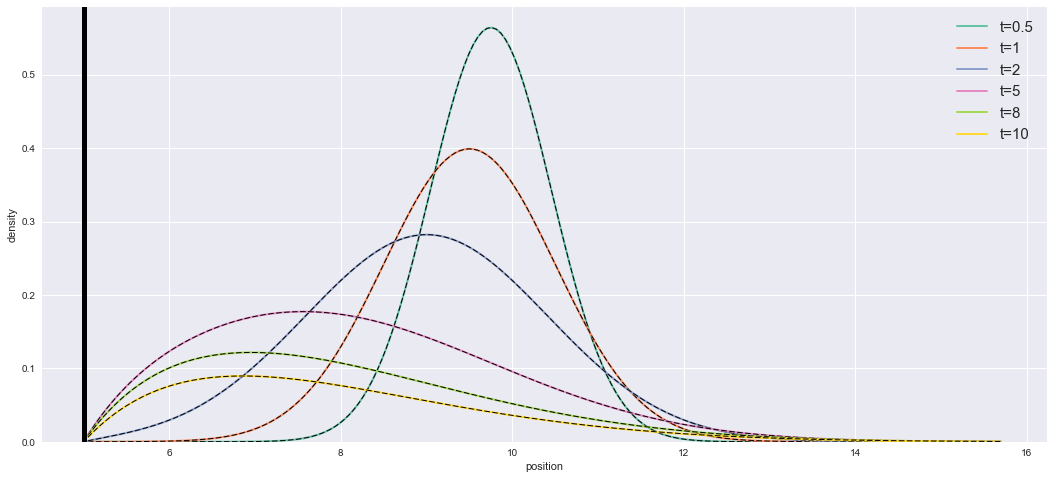
\includegraphics[width=\textwidth]{PDE_solution.png}
	\caption{We test the implementation of our PDE solver by considering the case of constant drift and volatility, $\mu(x) =  -0.5, ~\sigma = 1$, 
			initial condition $p(x, t=0) = \delta(x-10)$ and an absorbing barrier at $x=5$. 
			The black dashed lines on top of the colored lines indicates the analytical solution \eqref{eq:p_absorbing_explicit},
			in excellent agreement with the numerical one.}
	\label{fig:PDE_solution}
\end{figure}



%%%%%%%%%%%%%%%%%%%%%%%%%%%%%%%%%%%%%%%%%%%%%%%%%%%%%%%%%%%%%%%%
\clearpage
\bibliography{bibliography.bib}
\clearpage
%%%%%%%%%%%%%%%%%%%%%%%%%%%%%%%%%%%%%%%%%%%%%%%%%%%%%%%%%%%%%%%%



\section{Usage} 
%%%%%%%%%%%%%%%%%%%%%%%%%%%%%%%%%%%%%%%%%%%%%%%%%%%%%%%%%%%%%%%%%%



\end{document}